\lecture{19}{}{}

\begin{definition}
    Let $G$ be a group and $H$ be a subgroup of $G$. The \textit{left coset} of $H$ in $G$ is defined as:
    \[aH = \{ ah \mid h \in H \} \subseteq G\]
    for all $a \in G$. That is, all elements that is equivalent to a. \\
    Similarly, the \textit{right coset} of $H$ in $G$ is defined as:
    \[Ha = \{ ha \mid h \in H \} \subseteq G\]
    for all $a \in G$.\\
\end{definition}

\begin{eg}
    Let $G = \mathbb{Z}_{18} = \{0, 1, 2, \ldots, 17\}$ and $H = \langle 3 \rangle = \{0, 3, 6, 9, 12, 15\}$.\\
    Then the left cosets of $H$ in $G$ are: 
    \[0 + H = \{0, 3, 6, 9, 12, 15\}\]
    \[1 + H = \{1, 4, 7, 10, 13, 16\}\]
    \[2 + H = \{2, 5, 8, 11, 14, 17\}\]
    Note that $1 + H$ is not a subgroup of $G$.\\ 
\end{eg}

\begin{remark}
    We observe the following:
    \begin{enumerate}
        \item The left cosets of $H$ in $G$ partition $G$.
        \item $|H| = |1+H| = |2+H| = \ldots = |a+H|$ for all $a \in G$. (partitions have the same size)
    \end{enumerate}
\end{remark}

\begin{eg}
    Let $D_4 = \{e, \rho, \rho^2, \rho^3, \mu, \mu\rho, \mu\rho^2, \mu\rho^3\}$ be the dihedral group of permutation of a square.\\
    Let $H = \langle \mu \rho \rangle = \{e, \mu\rho\}$.\\
    Then the left cosets of $H$ in $D_4$ are: 
    \begin{center}
    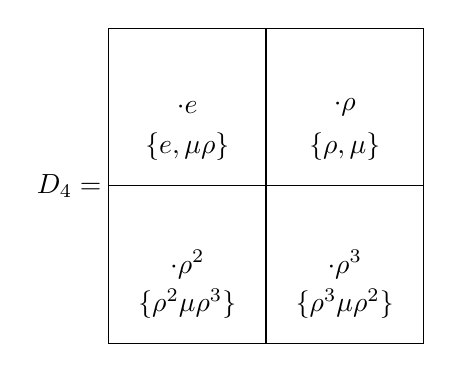
\begin{tikzpicture}
        \draw (0,0) rectangle (4,4);
        \draw (0,2) -- (4,2);
        \draw (2,0) -- (2,4);
        \node at (-0.5,2) {$D_4 =$};
        
        \node at (1,3) {$\cdot e$};
        \node at (1,2.5) {$\{e, \mu\rho\}$};
        
        \node at (3,3) {$\cdot \rho$};
        \node at (3,2.5) {$\{\rho, \mu\}$};
        
        \node at (1,1) {$\cdot \rho^2$};
        \node at (1,0.5) {$\{\rho^2 \mu\rho^3\}$};
        
        \node at (3,1) {$\cdot \rho^3$};
        \node at (3,0.5) {$\{\rho^3 \mu\rho^2\}$};
    \end{tikzpicture}
    \end{center}
\end{eg}

\begin{theorem}
    Let $G$ be a group and $H$ be a subgroup of $G$. Then for all $a \in G$, $|H| = |aH|$.
\end{theorem}
\begin{proof}
    Define a function $f : H \to aH$ by $f(x) = ax$. We show that $f$ is a bijection.
    \begin{enumerate}
        \item \textbf{one-to-one}: Suppose $f(h_1) = f(h_2)$. Then $ah_1 = ah_2 \implies h_1 = h_2$.
        \item \textbf{onto}: $y \in aH$ implies $y = ah$ for some $h \in H$. So $f(h) = ah = y$.
    \end{enumerate}
\end{proof}

\begin{prev}[Lagrange's Theorem]
    Recall:\\
    Let $G$ be a finite group and $H$ be a subgroup of $G$. Then $|H|$ divides $|G|$.\\
    Moreover, the number of left cosets of $H$ in $G$ is $\frac{|G|}{|H|}$.
\end{prev}
\begin{proof}
Let $G = \{a_1, a_2, \ldots, a_n\}$ and $H = \{h_1, h_2, \ldots, h_m\}$.\\
Then 
\[
G = \bigcup_{i=1}^n a_iH \quad \text{and} \quad a_iH \cap a_jH = \emptyset \text{ for } i \neq j.
\]
So 
\[
|G| = \sum_{i=1}^n |a_iH| = n|H|.
\]
Hence, $|H|$ divides $|G|$.
\end{proof}

\begin{eg}
    Let $G = \mathbb{Z}_{24} = \{0, 1, 2, \ldots, 23\}$ and $H = \langle 3 \rangle = \{0, 3, 6, \cdots, 21\}$.\\
    Then $|H| = 8$ and $|G| = 24$.\\
    So the number of left cosets of $H$ in $G$ is $\frac{24}{8} = 3$.\\
\end{eg}

\begin{exercise}
Let $S_5$ be the permutation group of 5 elements.\\
Let $\sigma \in S_5$ and $\sigma = (1, 2, 5, 4)(2, 3)$.\\
Find $(S_5, \langle \sigma \rangle)$.\\
\end{exercise}
\begin{answer}
    $(S_5, \langle \sigma \rangle) = \frac{|S_5|}{|\langle \sigma \rangle|} = \frac{5!}{|\langle \sigma \rangle|}$.\\
    $|\langle \sigma \rangle| = |(1, 2, 3, 5, 4)| = 5$.\\
    So $(S_5, \langle \sigma \rangle) = \frac{5!}{5} = 24$.\\
\end{answer}

\begin{exercise}
    Let $\phi : G \to G'$ be a group homomorphism.\\
    Show that $\phi(a) = \phi(b) \iff a^{-1}b \in Ker(\phi)$.
\end{exercise}
\begin{answer}
    ($\Rightarrow$) Suppose $\phi(a) = \phi(b)$. Then,
    \[\phi(a^{-1}b) = \phi(a^{-1})\phi(b) = \phi(a)^{-1}\phi(a) =  e\]
    So $a^{-1}b \in Ker(\phi)$.\\
\end{answer}